% Name: Convolution
% Description: A 3 by 3 kernel slid over a 5 by 5 input: the highlighted window, multiplied cell by cell with the kernel and summed, gives the highlighted output.
% Tags: convolution, kernel, feature map, CNN

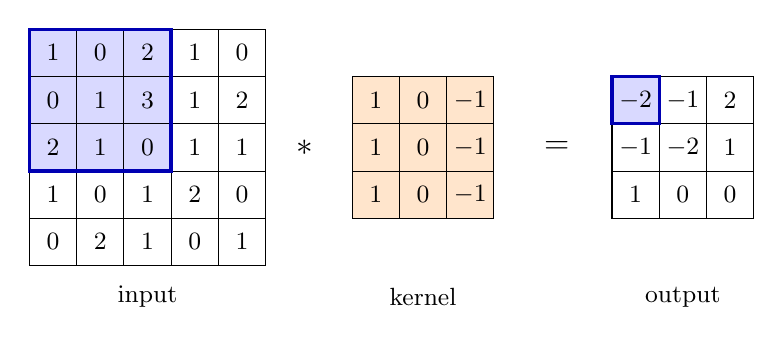
\begin{tikzpicture}[cell/.style={draw, minimum size=6mm, inner sep=0pt, font=\small}]
  % Output (r, c) is the sum over the window at (r, c) of input times kernel; the top-left is 1 + 0 + 2 - 2 - 3 + 0 = -2.
  \fill[blue!15] (0,0) rectangle (1.8,-1.8);
  \foreach \row [count=\r from 0] in {{1,0,2,1,0}, {0,1,3,1,2}, {2,1,0,1,1}, {1,0,1,2,0}, {0,2,1,0,1}}
    \foreach \v [count=\c from 0] in \row
      \node[cell] at (0.6*\c+0.3, -0.6*\r-0.3) {\v};
  \draw[very thick, blue!70!black] (0,0) rectangle (1.8,-1.8);
  \node[font=\large] at (3.5,-1.5) {$\ast$};
  \foreach \row [count=\r from 0] in {{1,0,-1}, {1,0,-1}, {1,0,-1}}
    \foreach \v [count=\c from 0] in \row
      \node[cell, fill=orange!20] at (0.6*\c+4.4, -0.6*\r-0.9) {$\v$};
  \node[font=\large] at (6.7,-1.5) {$=$};
  \fill[blue!15] (7.4,-0.6) rectangle (8,-1.2);
  \foreach \row [count=\r from 0] in {{-2,-1,2}, {-1,-2,1}, {1,0,0}}
    \foreach \v [count=\c from 0] in \row
      \node[cell] at (0.6*\c+7.7, -0.6*\r-0.9) {$\v$};
  \draw[very thick, blue!70!black] (7.4,-0.6) rectangle (8,-1.2);
  \node[font=\small] at (1.5,-3.4) {input};
  \node[font=\small] at (5,-3.4) {kernel};
  \node[font=\small] at (8.3,-3.4) {output};
\end{tikzpicture}
